\section{Only valid programs may run}
\label{sec:valid}

This section introduces the main syntactic categories of the language:
kinds, types, expressions, and programs. It also discusses type
equivalence.

\paragraph{Kinding validate typea}

\freest{} requires kinding; GV does not. And the reason lies on
polymorphism, not on context-free types.
%
\lstinline|!Int| is undoubtedly a session type, and so is
\lstinline|!Int;?Bool|. On the other hand, \lstinline|Int->Bool| and
\lstinline|(Int,Bool)| are certainly functional types. The GV language
allows a stratified grammar with separate syntactic categories for
functional types and for session types, even if mutually recursive.
%
In \freest{} this is not possible.  To see why, take for
\lstinline|alpha| a type variable. Is \lstinline|!Int;alpha| a
session type? What about \lstinline|alpha| itself? The former is a
session type only when \lstinline|alpha| represents a session type;
the latter is a functional type when \lstinline|alpha| denotes a
functional type, and is a session type otherwise. If \lstinline|alpha|
does not denote a session type, then \lstinline|!Int;alpha| is not a
type, it is simply a piece of useless syntax.

\begin{wrapfigure}{R}{0.12\textwidth}
  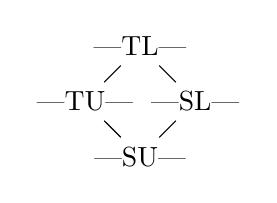
\begin{tikzpicture}[scale=.7]
    \node (TL) at (0,1) {\lstinline|TL|};
    \node (TU) at (-1,0) {\lstinline|TU|};
    \node (SL) at (1,0) {\lstinline|SL|};
    \node (SU) at (0,-1) {\lstinline|SU|};
    \draw (TL) -- (TU) -- (SU) -- (SL) -- (TL);
  \end{tikzpicture}
\end{wrapfigure}
%
To accommodate polymorphism, types are classified into \emph{kinds}.
%
% Kinds classify types. 
Kinds are pairs composed of a \emph{prekind} and a
\emph{multiplicity}. Prekinds distinguish functional types,
\lstinline|T|, from session types, \lstinline|S|.
%
Multiplicities control the number of times a value may be used in a
given context: exactly one---linear, \lstinline|L|---or zero or
more---unrestricted, \lstinline|U|. Both prekinds and multiplicities
come equipped with an ordering relation. Together they form the
lattice in the diagram on the right.
%
Types of kind \lstinline|TU| can be used at kind \lstinline|TL|. Also
types of kind \lstinline|SL| can be used at kind \lstinline|TL|.
Finally, any type can be seen of kind \lstinline|TL|, the kind sitting
at top of the hierarchy, the kind that carries the least information.

Equipped with kinds, \freest{} features as functional types the
following:
%
\begin{itemize}
\item The basic types, \lstinline|B : TU|, that is, \lstinline|Int|,
  \lstinline|Bool|, \lstinline|Char|, and \lstinline|()|,
\item Unrestricted and linear functions, \lstinline|T1 -> T2 : TU| and
  \lstinline|T1 -o T2 : TL|,
\item Unrestricted and linear pairs, \lstinline|<T1, T2> : TU| and
  \lstinline|(T1, T2) : TL|, and
\item Datatypes, \lstinline|[l1: T1, ..., ln: Tn]| of kind
  \lstinline|SU| or \lstinline|SL| depending on the kinds of the
  various types \lstinline|Ti|.
\end{itemize}

The session types are the following:
\begin{itemize}
\item The terminated type, \lstinline|Skip : SU|,
\item Sequential composition, \lstinline|S1;S2| of kind \lstinline|SU|
  or \lstinline|SL| depending on \lstinline|S1| and \lstinline|S2|,
\item  Messages, \lstinline|!B, ?B|, both of kind \lstinline|SL|,
\item Choices, \lstinline|+{l1: S1, ..., ln:Sn}, &{l1: S1, ..., ln:Sn}|,
  both of kind \lstinline|SL|,
\item Recursive types, \lstinline|rec x.S|, bearing the kind of
  \lstinline|S|.
\end{itemize}

\paragraph{One function, many forms}

We are now in a better position to understand the type signature for
the functions in Section~\ref{sec:programming}.  Polymorphic variables
are introduced solely with the \lstinline|forall| construct. The
non-abbreviated type for function \lstinline|treeSum| spells out the
kind for the polymorphic type variable \lstinline|alpha|, as follows:
%
\begin{lstlisting}
forall alpha:SL => Tree -> TreeC;alpha -> (Tree,alpha)
\end{lstlisting}
%
The absence of an explicit kind for a polymorphic variable is
understood as \lstinline|SL|. In this particular case, one can replace
\lstinline|alpha| by any type with kind \lstinline|SL| or smaller,
including types \lstinline|TreeC;?Int;alpha : SL| (line 8 in the code
for \lstinline|TreeSum| on Section~\ref{sec:programming}),
\lstinline|?Int;alpha : SL| (line 9), and \lstinline|Skip : SU| (line
25 in the code for \lstinline|main|).
%
The call to function \lstinline|transform| on line
8 effectively calls the function at type
%
\begin{lstlisting}
Tree -> TreeC;TreeC;?Int;alpha -> (Tree, TreeC;?Int;alpha).
\end{lstlisting}
%
making it clear that channel \lstinline|c| is supposed to convey two
trees (the left and the right subtrees of a non-empty tree) before it
produces an integer value. The function reads one tree from the
channel and returns the unused part of the channel, namely
\lstinline|TreeC;?Int;alpha|.

Because we declared \lstinline|alpha| of kind \lstinline|SL|,
functional types cannot replace \lstinline|alpha|.  If one tries to
replace \lstinline|alpha| by \lstinline|Int->Bool|, one would get
%
\lstinline|Tree -> TreeC;(Int->Bool) -> (Tree,Int->Bool)|, which is
not a well formed type for the semicolon operator is defined on
session types only.
%
At the time of this writing datatypes are monomorphic.

\paragraph{Repeated behavior}

A characteristic central to session types is their ability to describe
unbounded behavior, usually captured by recursive types. Recursion is
certainly useful in types such as \lstinline|TreeChannel| in
Section~\ref{sec:programming}, meant do describe channels able to
transmit binary trees of different sizes. We have seen that name
\lstinline|TreeC| abbreviates type
%
\lstinline|rec x. +{Leaf: Skip, Node: !Int;x;x;?Int}|.  Type variable
\lstinline|x|, monomorphic, belongs to kind \lstinline|SU| so that
type
%
\lstinline|+{Leaf: Skip, Node: !Int;x;x;?Int}| may be deemed well
formed (and of kind \lstinline|SL|).
%
Recursive types must be \emph{contractive} or free from unguarded
recursion. The following types are not contractive:
%
\lstinline|rec x1. ... rec xn.x1| and
%
\lstinline|rec x1. ... rec xn.(x1;S)|, for \lstinline|n>1| and for any
session type \lstinline|S|.
%
Only session types can be recursive. Recursion in the functional part
of the type language is obtained via datatypes as usual.

\paragraph{Expressions}

\freest{} blends expressions typical of functional languages and of
session types. In a way, it is not much different from GV.
%
The expressions inspired from functional languages include:
%
\begin{itemize}
\item Basic values: characters, integer and boolean values, and the
  unit value, \lstinline|()|,
\item Term variables (as opposed to type variables),
\item Lambda introduction, \lstinline|\x -o E| for linear abstractions
  and \lstinline|\x -> E| for unrestricted abstractions, and
  elimination, \lstinline|E1 E2|,
\item Pair introduction, \lstinline|(E1,E2)|, and elimination,
  \lstinline|let x, y = E1 in E2| (linear versions only, at the time
  of this writing),
\item Datatype elimination,
  \lstinline|case E of C1 x11...x1k -> E1, ..., Cn xn1...xnk -> En|, and
\item Conditional, \lstinline|if E1 then E2 else E3|, type
  application, \lstinline|x[T1,...Tn]|, and thread creation,
  \lstinline|fork E|.
\end{itemize}

The session-type related expression are:
%
\begin{itemize}
\item Channel creation, \lstinline|new S|,
\item Message send and reception, \lstinline|send E| and
  \lstinline|receive E|, and
\item Branch selection, \lstinline|select C E|, and match,
  \lstinline|match E with C1 x -> E1,...,Cn -> En|.
\end{itemize}

\paragraph{Programs}

Programs are composed of
%
\begin{itemize}
\item Function signatures and function declarations, 
\item Datatype declarations,
\item Type abbreviations.
\end{itemize}

Both functions and datatypes can be mutually recursive. Haskell code
is generated for programs that contain a function named
\lstinline|main| with a non-function type. The result of the
evaluation of this function is printed on the console.

%%% Local Variables:
%%% mode: latex
%%% TeX-master: "main"
%%% End
